\documentclass[margin=1cm]{standalone}
\usepackage{tikz}
\begin{document}
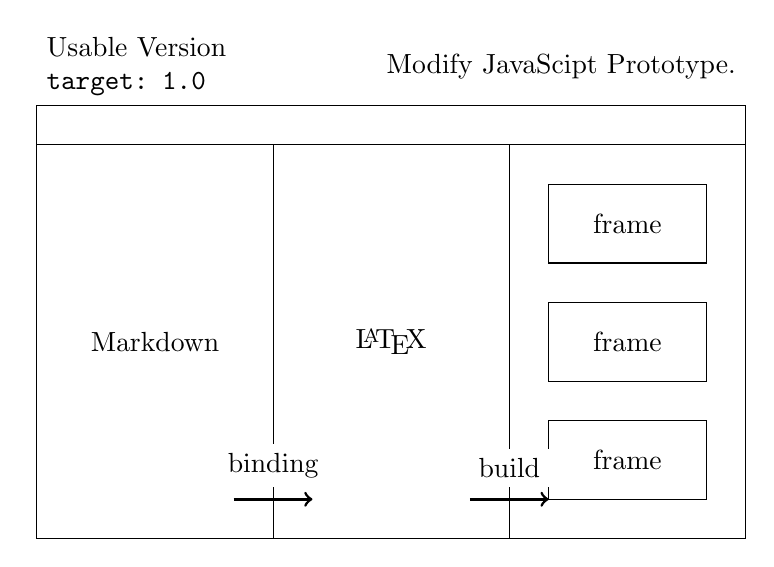
\begin{tikzpicture}
\draw  (2.5,3) rectangle (5.5,-2);
\draw  (-0.5,-2) rectangle (-3.5,3) node (v1) {};
\draw  (2.5,-2) rectangle (-0.5,3);
\draw  (3,2.5) rectangle (5,1.5);
\draw  (3,1) rectangle (5,0);
\draw  (3,-0.5) rectangle (5,-1.5);
\node at (-2,0.5) {Markdown};
\node at (1,0.5) {\LaTeX{}};
\node at (4,2) {frame};
\node at (4,0.5) {frame};
\node at (4,-1) {frame};
\draw [line width=1pt] (-1,-1.5) edge [->] node [above,fill=white, yshift=4pt] {binding} (0,-1.5);
\draw [line width=1pt] (2,-1.5) edge [->] node [above,fill=white, yshift=4pt] {build} (3,-1.5);
\node [right, text width=8em] at (-3.5,4) {Usable Version \texttt{target: 1.0}};
\draw  (v1) rectangle (5.5,3.5);
\node [left] at (5.5,4) {Modify JavaScipt Prototype.};
\end{tikzpicture}
\end{document}